\chapter{Implementation}

    \paragraph*{}
        The Application was mainly implemented in TypeScript. Implementation was done using React and Ionic.

        \begin{table}[htb]
            \centering
            \begin{tabular}{ | l | c | }
                \hline
                 & Technologies used \\
                \hline
                \hline
                Frontend & React \\ 
                \hline
                Backend & Node.js \\
                \hline
                API & REST\\
                \hline
                Database & MongoDb\\
                \hline
                OTP & Firebase  \\
                \hline
                Chat & Socket.io \\
                \hline
            \end{tabular}
            \caption{Technologies Used}
            \label{tab:Technologies}
        \end{table}


    \section{Frontend}

    React with TypeScript was used for the frontend. Redux was used to store the state of the application and use it throughout frontend.
        
    \subsection{API Key}
    The API key to communicate with the Google Maps APIs is in the environment variable. This is done in the .env file.
        \begin{figure}[h]
            \centering
            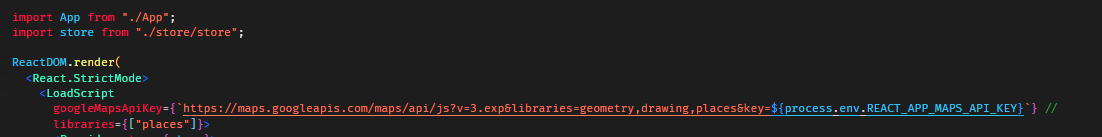
\includegraphics[width=0.8\textwidth]{images/APIkey.png}
            \caption{API Key}
            \label{fig:API}
        \end{figure}

    \pagebreak

    \subsection{Store}
    The store is the main data storage for the application. It uses redux which in turn uses different slices to store information.
    \begin{figure}[h]
        \centering
        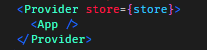
\includegraphics[width=0.5\textwidth]{images/redux_store.png}
        \caption{Store Provider}
        \label{fig:redux_store}
    \end{figure}

    % \pagebreak

    \subsection{Store Slice}
    The store slice is used through the reducers defined in the slice. Each Slice is given a name and a initial value. In this case the initial value is an empty object and the name of the slice is User. 
    \begin{figure}[h]
        \centering
        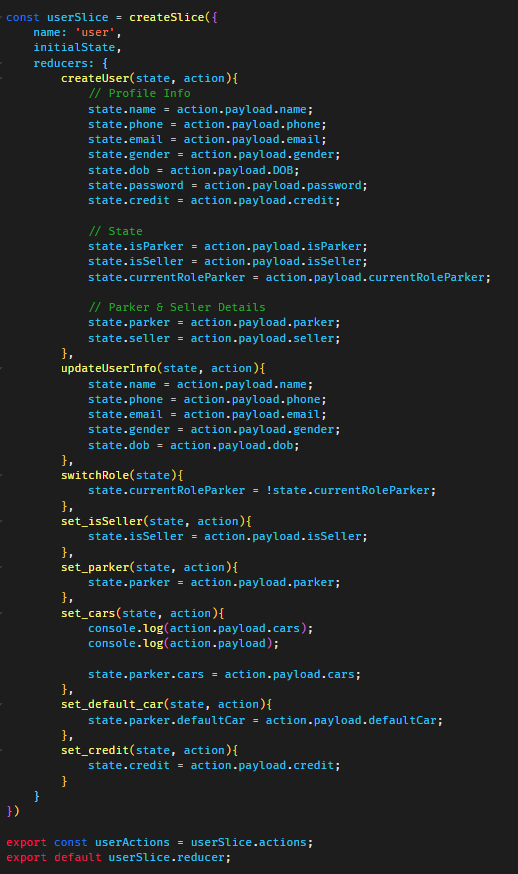
\includegraphics[width=0.425\textwidth]{images/storeSlice.png}
        \caption{User Slice in Store}
        \label{fig:storeSlice}
    \end{figure}

    \pagebreak


    \subsection{Routing}
    Routing on the Frontend is done using React Router 6. All the routes are defined in the App.tsx
    \begin{figure}[h]
        \centering
        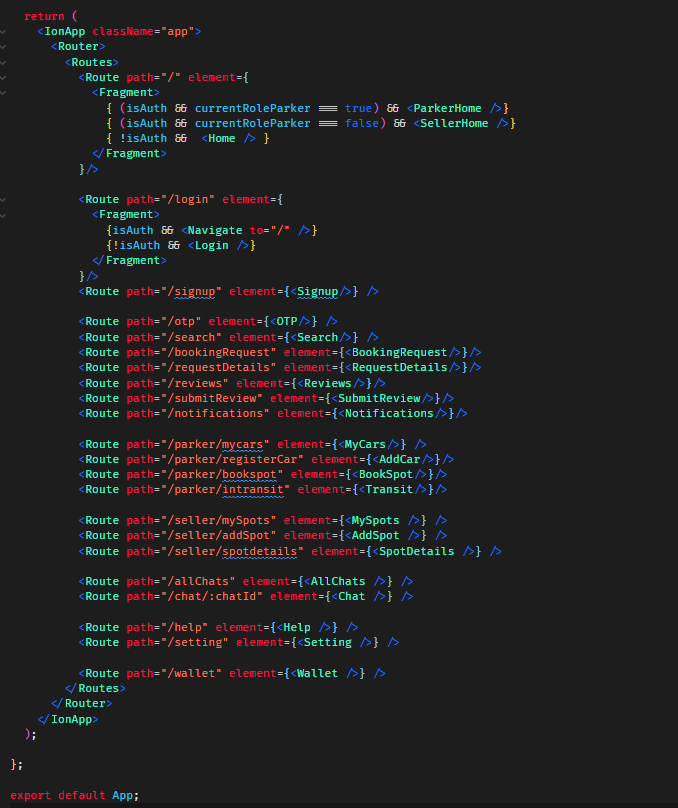
\includegraphics[width=0.7\textwidth]{images/routes.png}
        \caption{Routes}
        \label{fig:routes}
    \end{figure}

    \pagebreak

    \subsection{Firebase and Authentication}
    After a user registers on the application a OTP is sent to the user's number to verify their identity. The OTP is sent using Firebase's Authentication API.

    \begin{figure}[h]
        \centering
        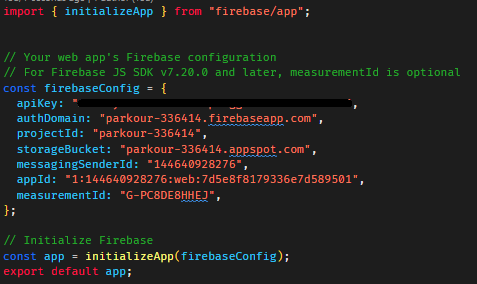
\includegraphics[width=0.7\textwidth]{images/firebaseConfig.png}
        \caption{Firebase Config}
        \label{fig:firebaseConfig}
    \end{figure}

    \pagebreak

    \subsection{Structure}
    Folder Structure used in the application.
    \begin{figure}[h]
        \centering
        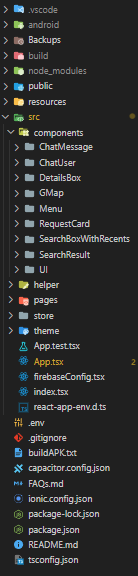
\includegraphics[width=0.2\textwidth]{images/folderStructure.png}
        \caption{Folder Structure in React}
        \label{fig:folderStructure}
    \end{figure}

    \pagebreak


    \subsection{Configuring Google Map}
    Google Map was configured in the Map.tsx file using the Google Maps API that was defined in Fig. \ref*{fig:API}.

    \begin{figure}[h]
        \centering
        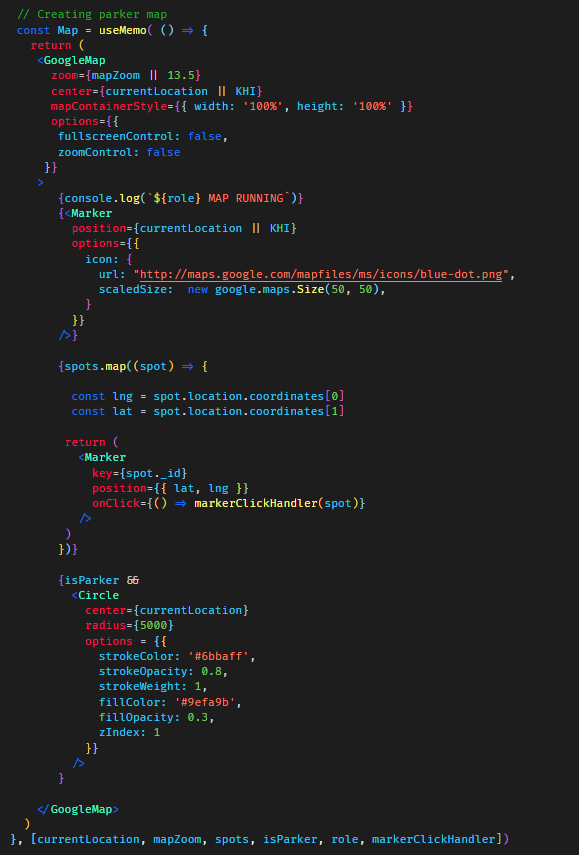
\includegraphics[width=0.6\textwidth]{images/googleMap.png}
        \caption{Google Map Configuration}
        \label{fig:googleMap}
    \end{figure}

    \pagebreak


    \section{Backend}

    Node.js and Express was used to communicate with the frontend and Express provides Express Router which was used to create proper routing for APIs.
        
    \subsection{Database Connection}
    The connection was done using the Mongoose library. The server starts when the connection is established.
        \begin{figure}[h]
            \centering
            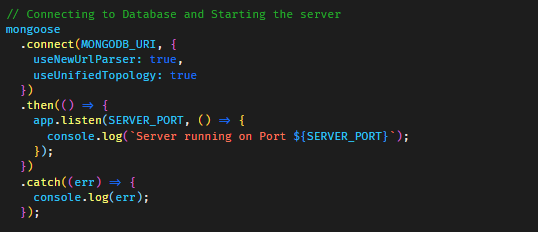
\includegraphics[width=0.8\textwidth]{images/dbConnection.png}
            \caption{Database Connection}
            \label{fig:dbConnection}
        \end{figure}

    \pagebreak

    \subsection{API Routes}
        All the Routes are established in the App.js which is also the entry point in our application.
    \begin{figure}[h]
        \centering
        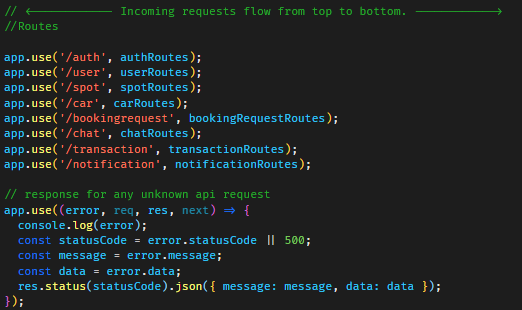
\includegraphics[width=0.8\textwidth]{images/BE_Routes.png}
        \caption{API Routes}
        \label{fig:BE_Routes}
    \end{figure}

    \pagebreak

    \subsection{Sockets}
    The sockets were used to communicate with the frontend. The sockets were used to enable bi-directional conversation to the frontend.\\

    \begin{figure}[h]
        \centering
        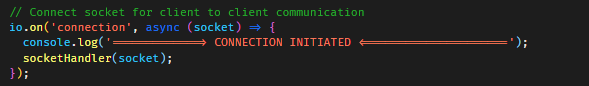
\includegraphics[width=0.8\textwidth]{images/socketConnection.png}
        \caption{Socket Connection}
        \label{fig:socketConnection}
    \end{figure}

    \subsection{Chat Server}
    Chat Server uses sockets and is run differently from the main server. Chat Server emits and receives events through sockets.
    \begin{figure}[h]
        \centering
        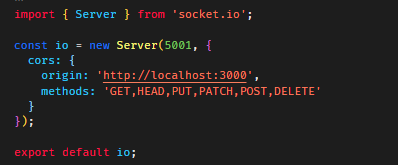
\includegraphics[width=0.8\textwidth]{images/chatServer.png}
        \caption{Chat Server}
        \label{fig:chatServer}
    \end{figure}

    \pagebreak


    \subsection{Routing}
    Routing on the Backend is done using Express Router. Here is an example of routing that is done for each module.
    \begin{figure}[h]
        \centering
        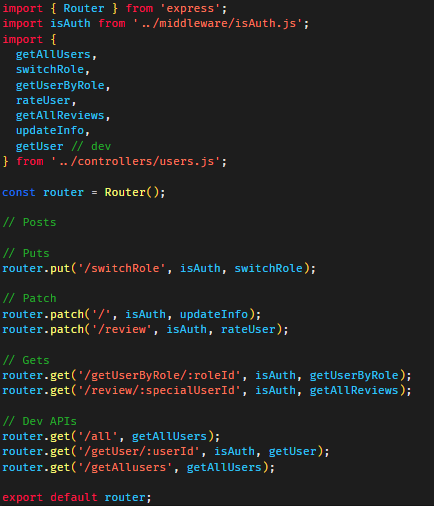
\includegraphics[width=0.8\textwidth]{images/user_Routes.png}
        \caption{User Routes}
        \label{fig:user_Routes}
    \end{figure}

    \pagebreak

    \subsection{Middleware}
        Middleware are used to reduce duplication in code and to make the code more readable. This also helps with filtering out the invalid API calls.
    \begin{figure}[h]
        \centering
        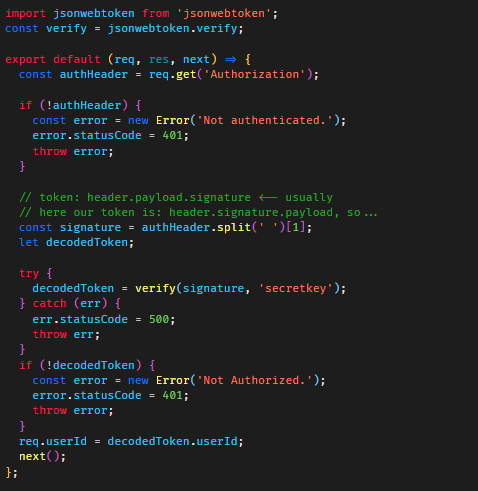
\includegraphics[width=0.8\textwidth]{images/isAuth.png}
        \caption{isAuth Middleware}
        \label{fig:isAuth}
    \end{figure}

    \pagebreak

    \subsection{Controllers}
    Controllers are used to save and retrieve data from the database. Controllers are used to handle the requests from the frontend and after the request is handled with appropriate calculation, the response is sent to the frontend.

    \begin{figure}[h]
        \centering
        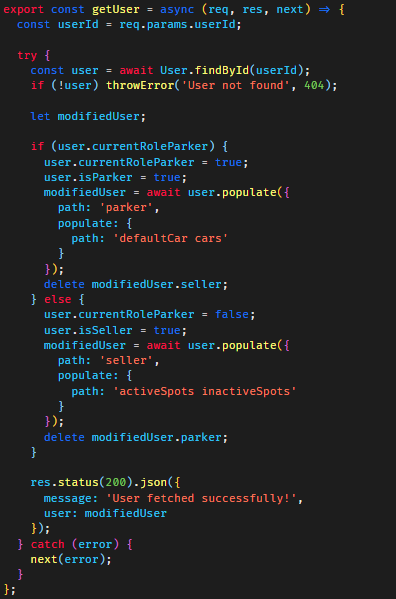
\includegraphics[width=0.6\textwidth]{images/userController.png}
        \caption{User Controller}
        \label{fig:userController}
    \end{figure}

    \pagebreak


    \section{Database}
    \subsection{Models}
    \paragraph*{}
        It is important to highlight the models that were designed and used.
        Each model had been given a careful consideration to make sure that the model is as modular as possible. The models were designed to be able to be used in multiple ways.The models were also designed in such a way that it will reduce redundancy wherever possible.\\

        \begin{figure}[h]
            \centering
            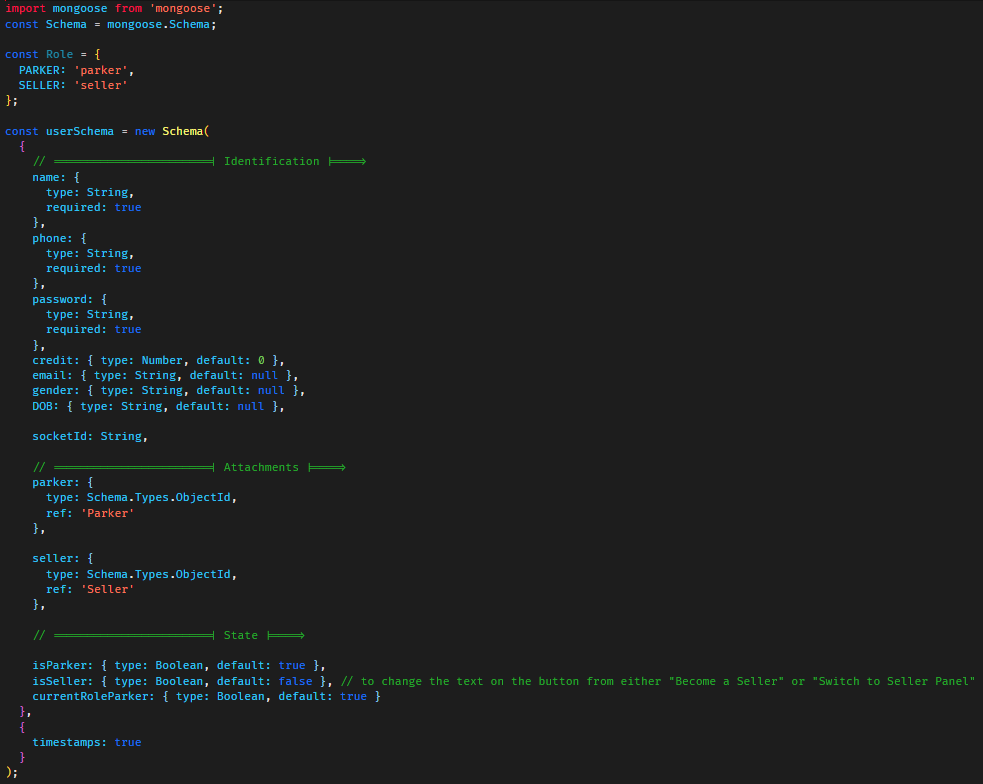
\includegraphics[width=0.6\textwidth]{images/userModel.png}
            \caption{User Model}
            \label{fig:userModel}
        \end{figure}

        \begin{figure}[h]
            \centering
            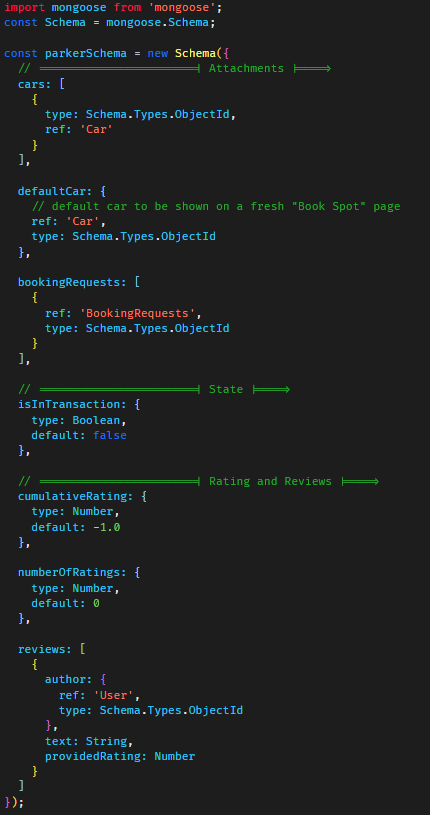
\includegraphics[width=0.65\textwidth]{images/parkerModel.png}
            \caption{Parker Model}
            \label{fig:parkerModel}
        \end{figure}


        \begin{figure}[h]
            \centering
            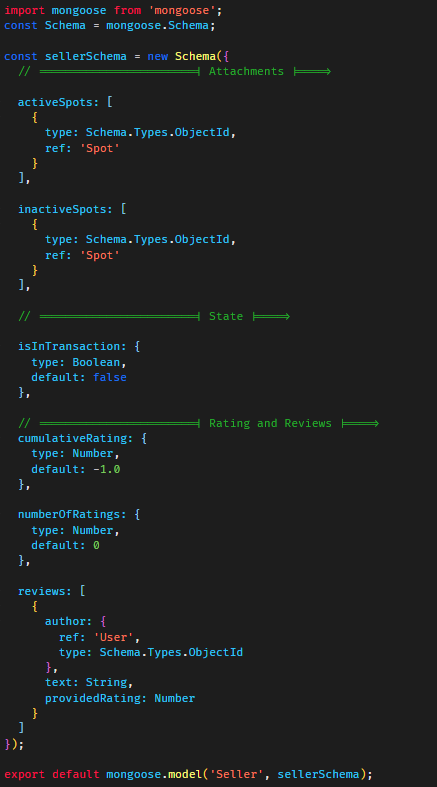
\includegraphics[width=0.65\textwidth]{images/sellerModel.png}
            \caption{Seller Model}
            \label{fig:sellerModel}
        \end{figure}

        \begin{figure}[h]
            \centering
            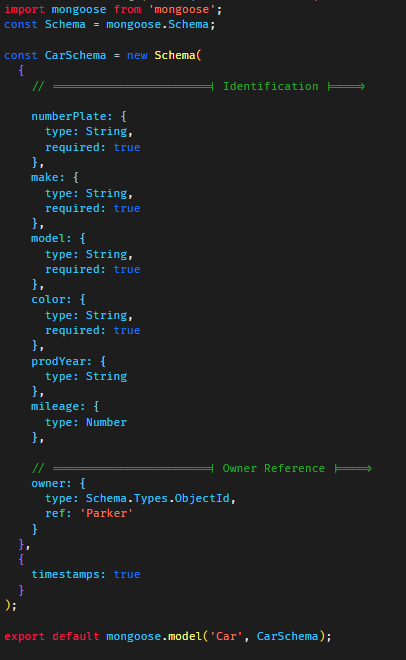
\includegraphics[width=0.7\textwidth]{images/carsModel.png}
            \caption{Car Model}
            \label{fig:carsModel}
        \end{figure}

        \begin{figure}[h]
            \centering
            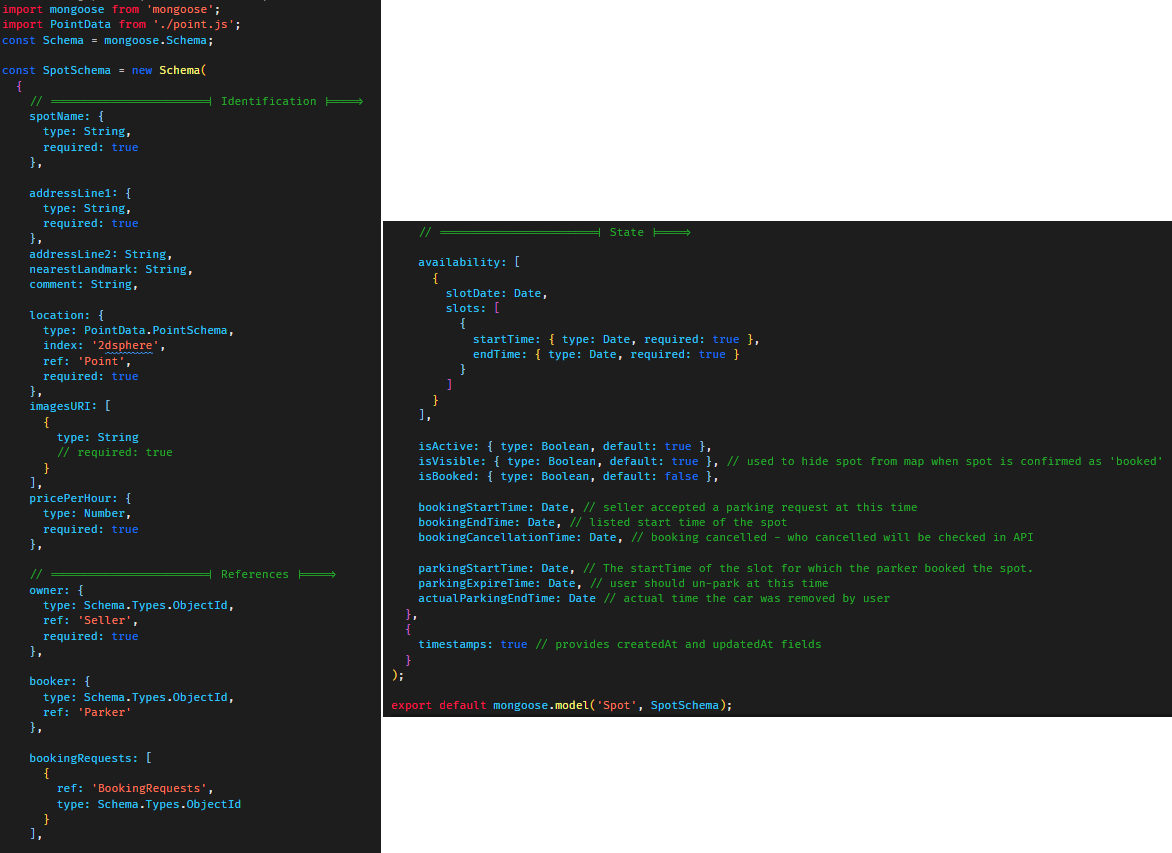
\includegraphics[width=1\textwidth]{images/spotModel.png}
            \caption{Spots Model}
            \label{fig:spotModel}
        \end{figure}

        \begin{figure}[h]
            \centering
            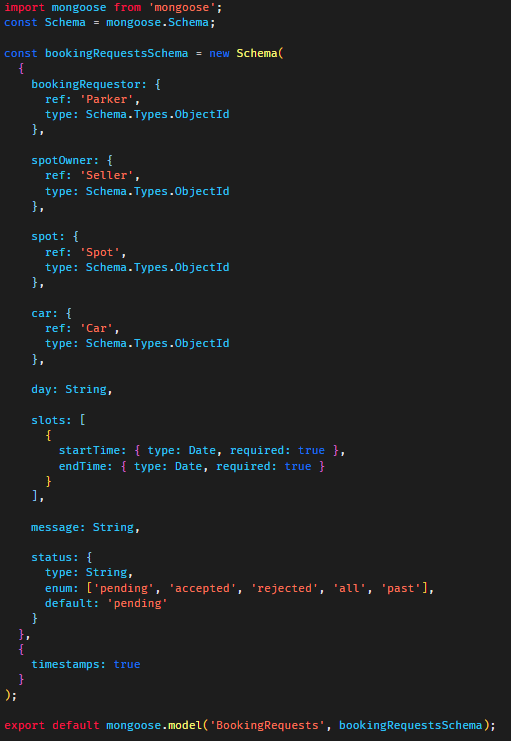
\includegraphics[width=0.8\textwidth]{images/bookingModel.png}
            \caption{Booking Request Model}
            \label{fig:bookingModel}
        \end{figure}


        \begin{figure}[h]
            \centering
            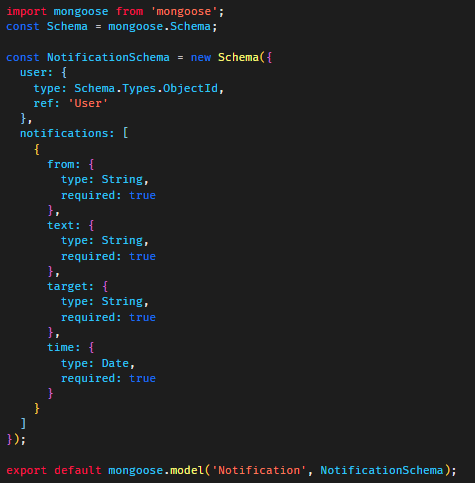
\includegraphics[width=0.8\textwidth]{images/notificationModel.png}
            \caption{Notification Model}
            \label{fig:notificationModel}
        \end{figure}


        \begin{figure}[h]
            \centering
            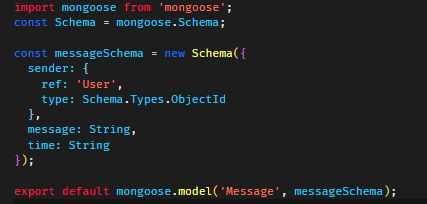
\includegraphics[width=0.8\textwidth]{images/messageModel.png}
            \caption{Message Model}
            \label{fig:messageModel}
        \end{figure}


        \begin{figure}[h]
            \centering
            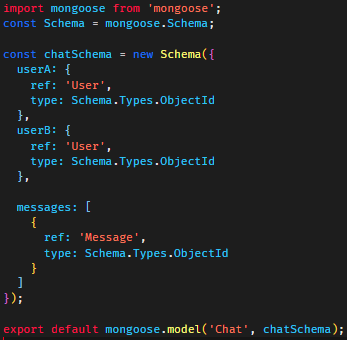
\includegraphics[width=0.8\textwidth]{images/chatModel.png}
            \caption{Chat Model}
            \label{fig:chatModel}
        \end{figure}


    \pagebreak
    \clearpage

    \section{Behavior}
    A list of the behavior that was implemented in the Application. This also includes the flow of the application.

    \subsection{Parker}
        The Behavior of the Parker is as follows
        \begin{figure}[h]
            \centering
            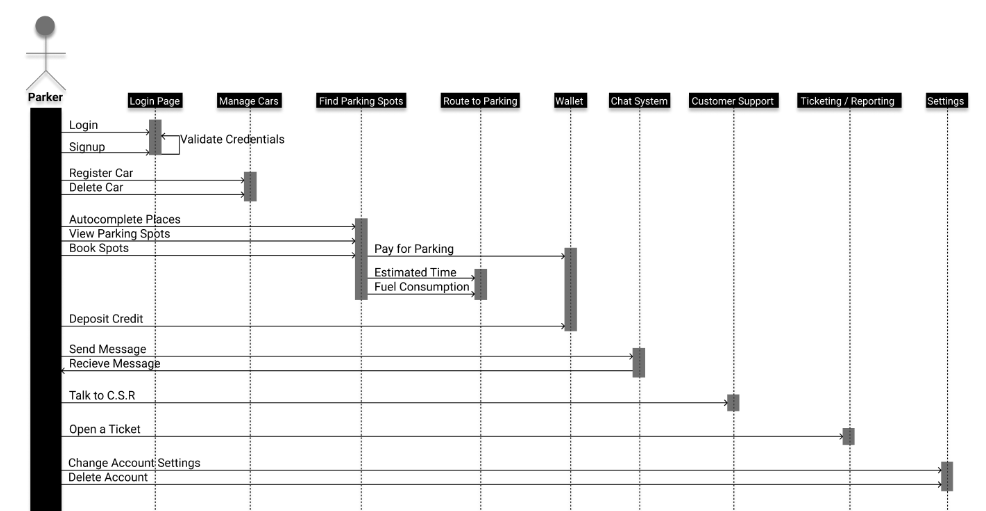
\includegraphics[width=1\textwidth]{images/parkerBehaviour.png}
            \caption{Parker Behavior (1)}
            \label{fig:parkerBehavior}
        \end{figure}

        % \pagebreak

        \begin{figure}[h]
            \centering
            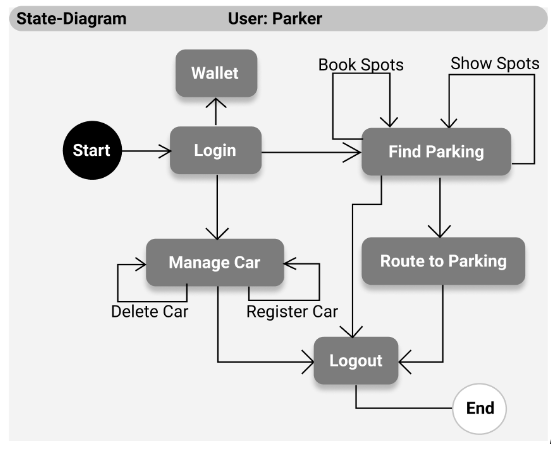
\includegraphics[width=1\textwidth]{images/parkerBehaviour2.png}
            \caption{Parker Behavior (2)}
            \label{fig:parkerBehavior2}
        \end{figure}

        \pagebreak
        \clearpage
        

    \subsection{Seller}
        The Behavior of the Seller is as follows
        \begin{figure}[h]
            \centering
            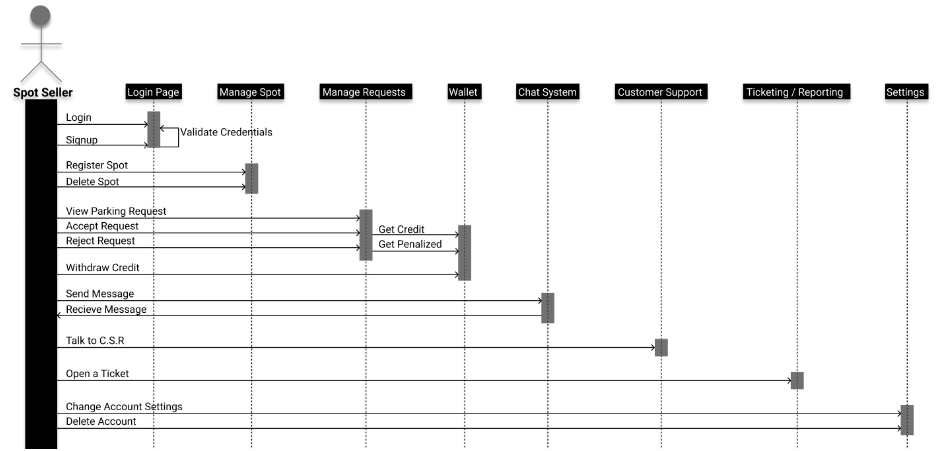
\includegraphics[width=1\textwidth]{images/sellerBehaviour.png}
            \caption{Seller Behavior (1)}
            \label{fig:sellerBehaviour}
        \end{figure}

        \pagebreak

        \begin{figure}[h]
            \centering
            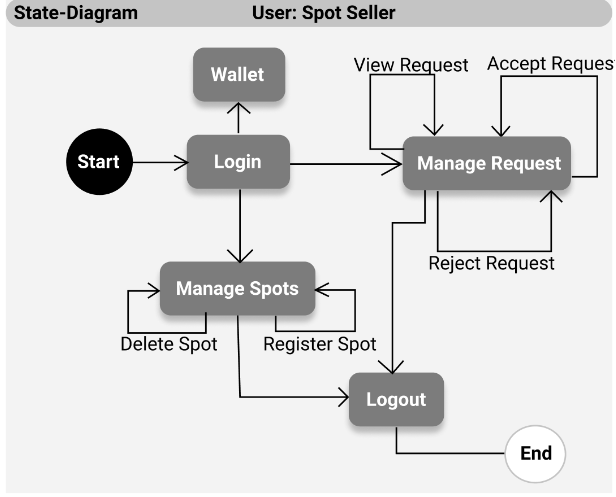
\includegraphics[width=1\textwidth]{images/sellerBehaviour2.png}
            \caption{Seller Behavior (2)}
            \label{fig:sellerBehaviour2}
        \end{figure}


    \pagebreak

    \subsection{Spot}
        The Behavior of the Spot is as follows
        \begin{figure}[h]
            \centering
            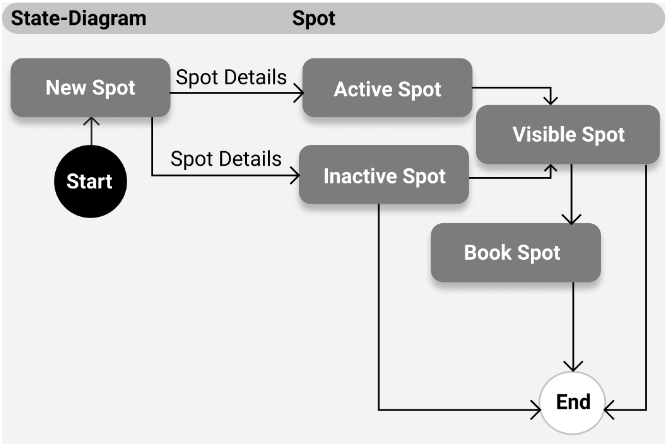
\includegraphics[width=1\textwidth]{images/spotBehaviour.png}
            \caption{Spot Behavior}
            \label{fig:spotBehaviour}
        \end{figure}


    \pagebreak

    \subsection{Booking Request}
        The Behavior of the Booking Request is as follows
        \begin{figure}[h]
            \centering
            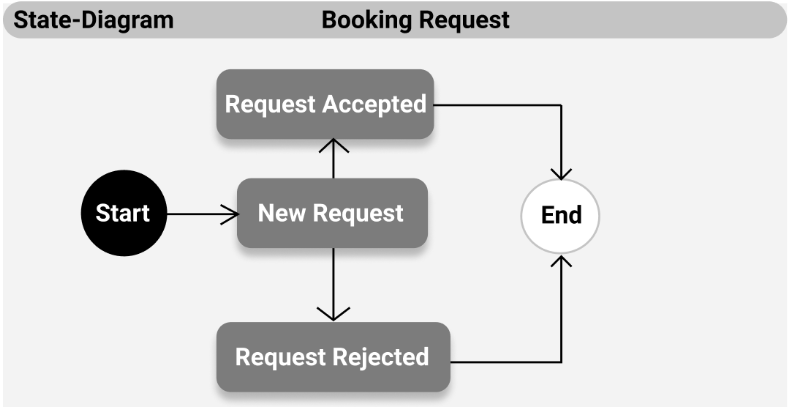
\includegraphics[width=1\textwidth]{images/bookingRequestBehaviour.png}
            \caption{Booking Request Behavior}
            \label{fig:bookingRequestBehaviour}
        \end{figure}

    \pagebreak